\documentclass[aspectratio=169,10pt]{beamer}
\usetheme{default}
\usecolortheme{seahorse}
\setbeamertemplate{navigation symbols}{}
\setbeamertemplate{footline}[frame number]
\usepackage{graphicx, booktabs, siunitx}
\graphicspath{{../figures/}}

\title{Imaging the Plastics on the SiPM Wall $\rightarrow$ a Geometry Calibration}
\subtitle{n\_TOF EAR2 X17 --- run 224404, MIP coincidences + Geant4 geometry}
\author{Dylan Neff \\[0.5ex] {\small analysis and slides prepared with Claude (Anthropic AI assistant)}}
\date{July 17, 2026}

\begin{document}

\begin{frame}\titlepage\end{frame}

\begin{frame}{Idea: no fitted energy scale needed --- use the geometry}
\begin{columns}
\column{.56\textwidth}
\begin{itemize}
\item Take the wall--plastic coincidences, \textbf{assume they are MIPs},
      and \textbf{assume they come from the source} (He-3 target at the origin).
\item Geometry from the Geant4 sim (\texttt{mx17\_geom.py}): bars run \emph{along}
      the beam (+Y), wall at $R\!\approx\!33$ cm, plastics behind at $R\!\approx\!43$ cm.
\item A source track hits the wall at angle $\theta$, so a MIP deposits
      $E=\frac{dE}{dx}\cdot\frac{t_{\rm scint}}{\cos\theta}$ in the 3 mm bar.
\item Two consequences:
  \begin{enumerate}
    \item each plastic \emph{projects} onto the wall $\Rightarrow$ imaging;
    \item the MIP peak must scale as $1/\cos\theta$ $\Rightarrow$ a calibration.
  \end{enumerate}
\end{itemize}
\column{.44\textwidth}
\centering
$\cos\theta = R_{\rm wall}/\sqrt{R_{\rm wall}^2+u^2+v^2}$\\[1ex]
plastic $\to$ wall projection scale\\ $R_{\rm wall}/R_{\rm plastic}=0.77$\\[1ex]
$\Rightarrow$ geo-mean MIP peak $\propto$ gain $\times \dfrac{1}{\cos\theta}$
\end{columns}
\end{frame}

\begin{frame}{Geometry: the two projections and the coordinates}
\centering
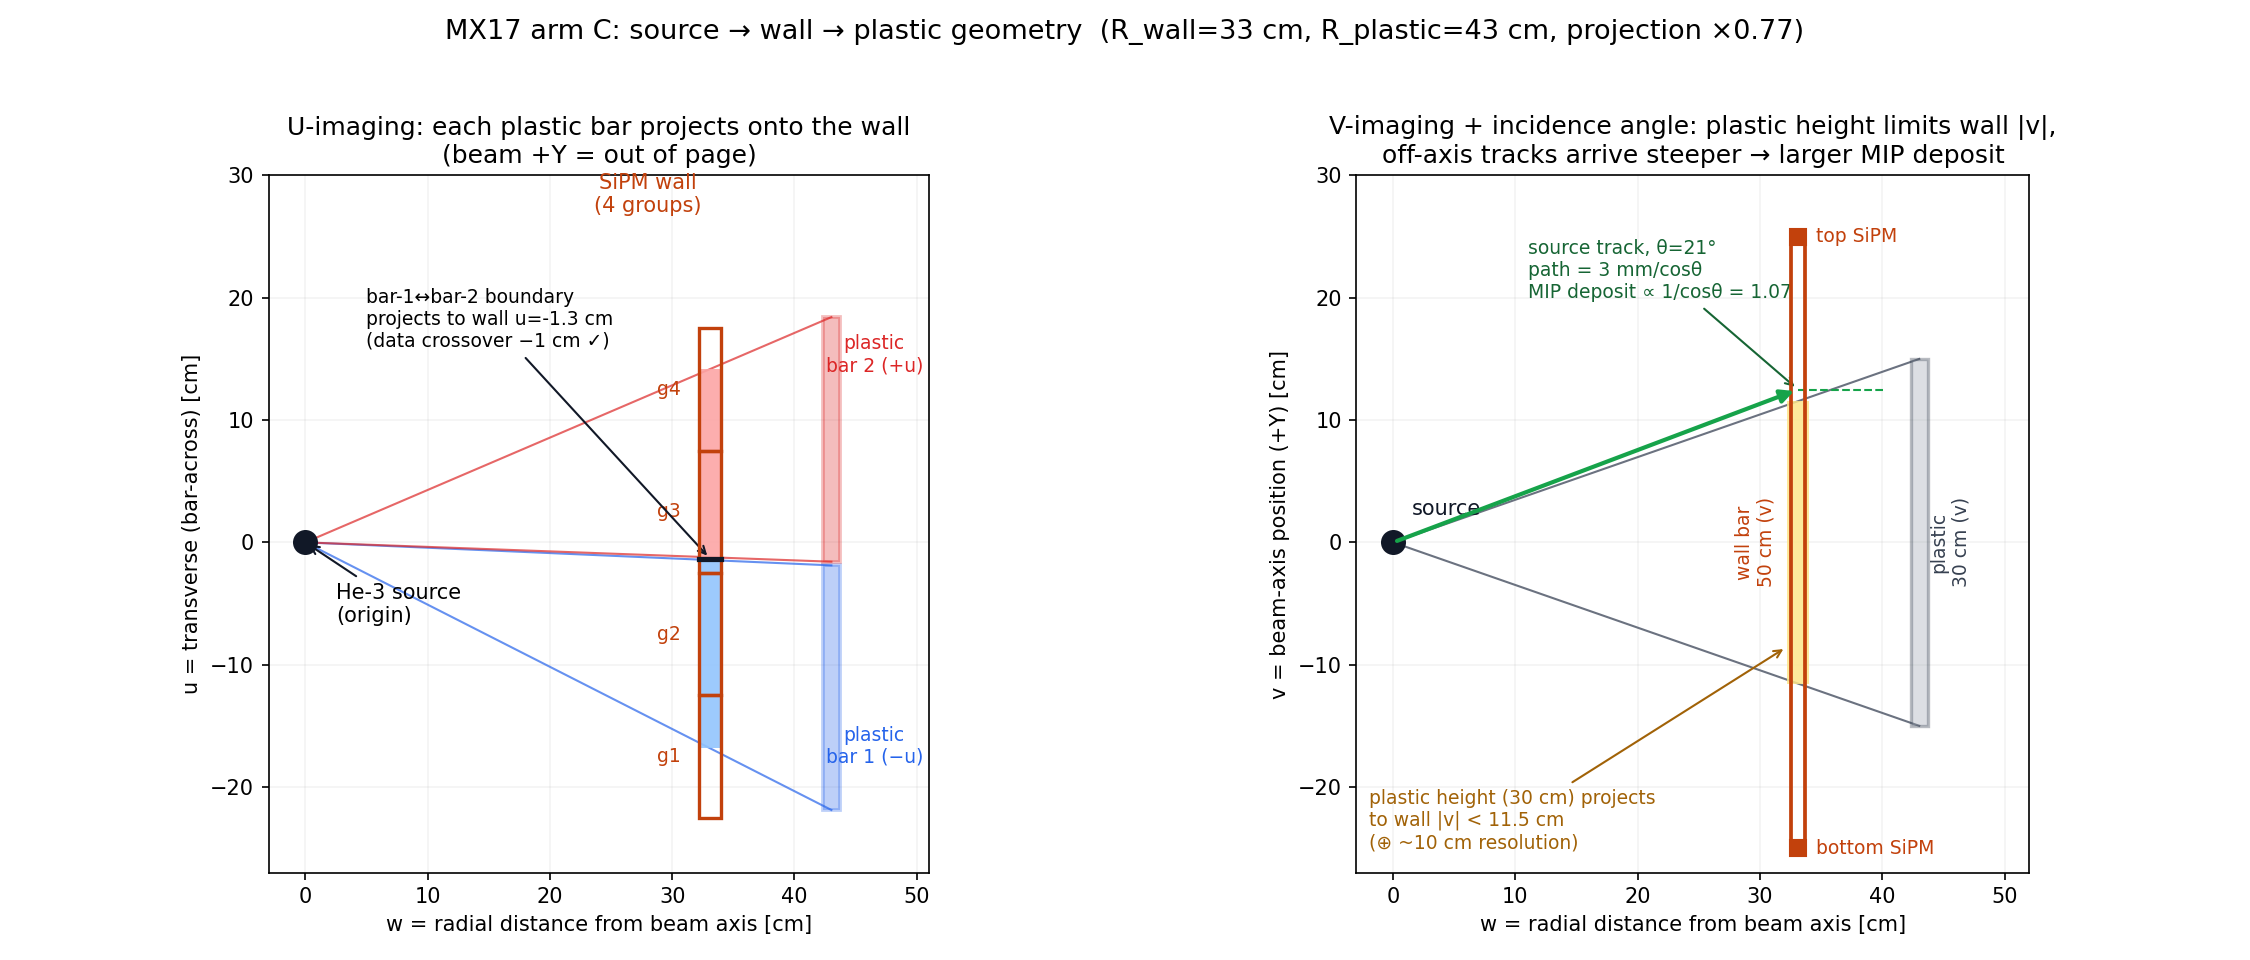
\includegraphics[width=\textwidth]{17_imaging/geometry_diagram.png}\\
{\footnotesize \textbf{u} = transverse (bar-across), \textbf{v} = beam axis (+Y,
bar length, read top/bottom), \textbf{w} = radial. \emph{Left:} rays from the
source through each plastic bar illuminate different wall groups (blue bar-1$\to$g1,2;
red bar-2$\to$g3,4). \emph{Right:} the plastic height limits the wall $|v|$, and an
off-axis track arrives at angle $\theta$ $\Rightarrow$ longer path $\Rightarrow$
larger MIP deposit.}
\end{frame}

\begin{frame}{Imaging: the wall sees the plastics from the source}
\centering
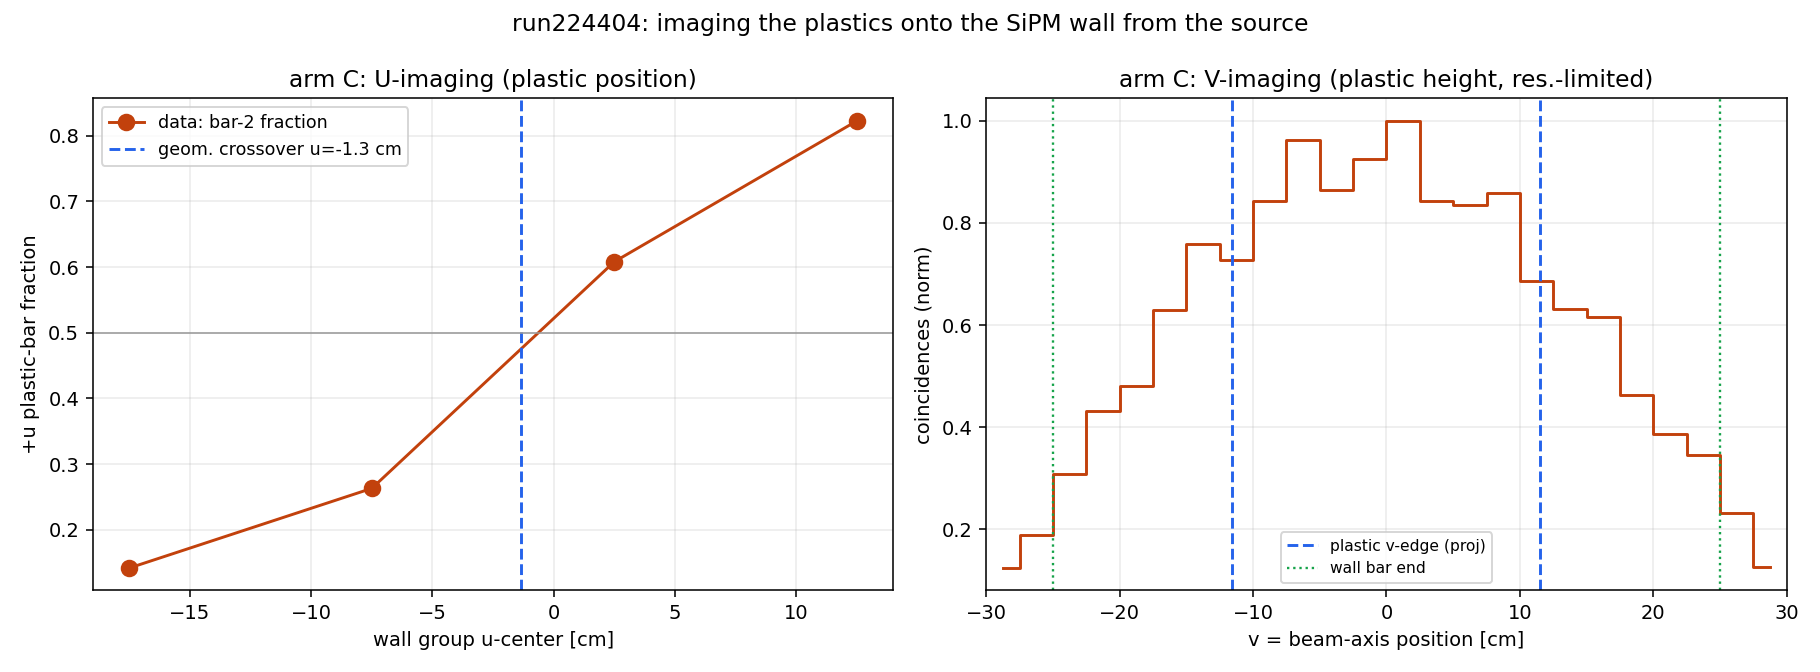
\includegraphics[width=\textwidth]{17_imaging/imaging_C.png}\\
{\footnotesize \textbf{Left (U):} fraction of coincidences tagged by the $+u$
plastic bar climbs monotonically across the wall groups, crossing 50\% at
$u\!\approx\!-1$ cm --- exactly the source-projected plastic-bar boundary
($-1.3$ cm). \emph{The tracks really do come from the source.} \textbf{Right (V):}
coincidences centre at $v=0$ and fall off near the projected plastic height
($\pm$11.5 cm); the soft edges are the $\sim$10 cm timing/amplitude resolution.}
\end{frame}

\begin{frame}{Calibration: correct the MIP peak by $1/\cos\theta$}
\centering
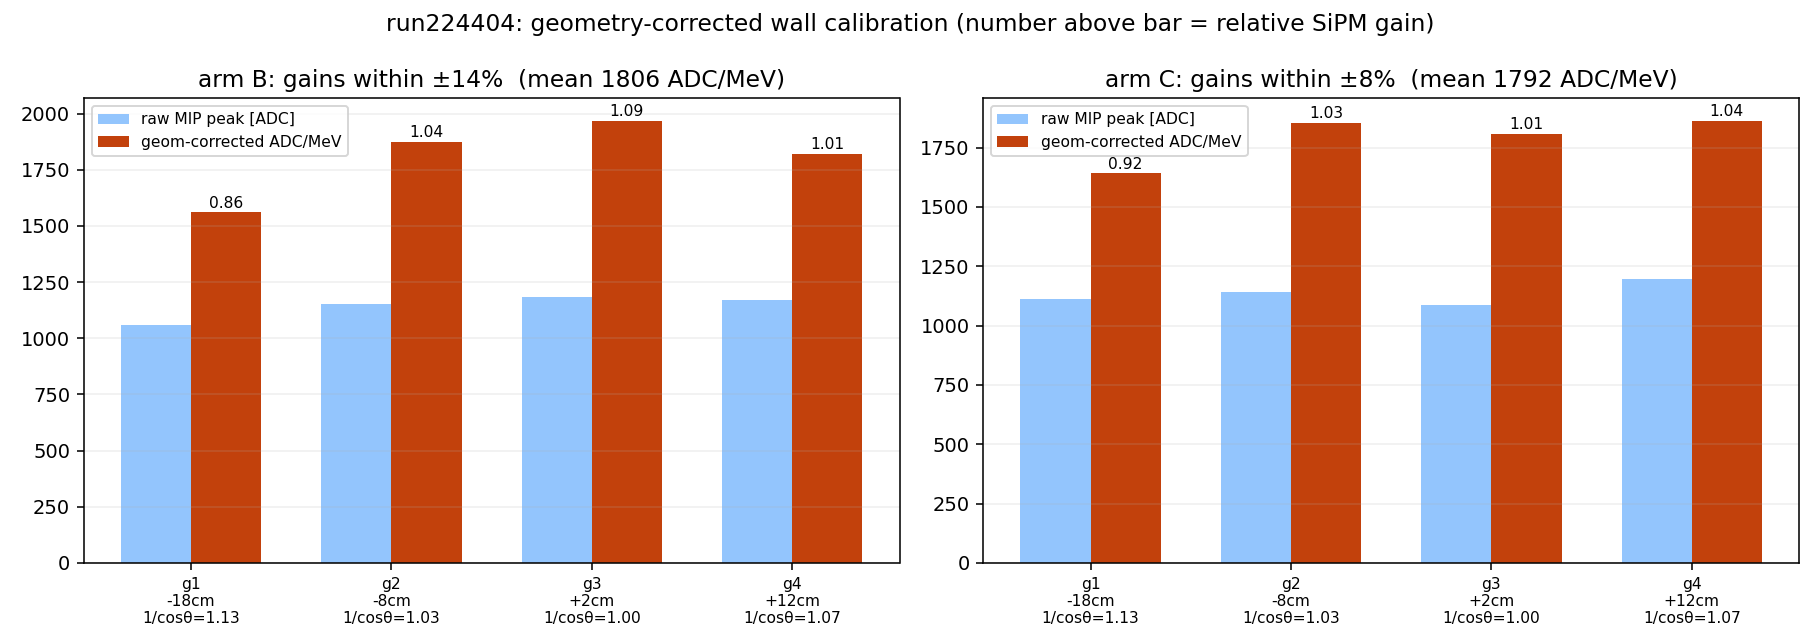
\includegraphics[width=\textwidth]{17_imaging/calibration_bars.png}\\
{\footnotesize Raw MIP peak (blue) is nearly flat across the wall; dividing by the
geometric deposit $E=0.6\,\text{MeV}/\cos\theta$ gives \textbf{ADC/MeV}
(orange). Per-group \textbf{relative SiPM gain} (numbers) sits within
$\pm$8--14\%; group 1 (far $-u$ edge) is $\sim$10\% low on both arms. Mean
$\approx$1800 ADC/MeV.}
\end{frame}

\begin{frame}{What this gives --- and its limits}
\begin{itemize}
\item \textbf{Geometry \& source confirmed} by the U-imaging (bar-fraction gradient
      matches the projected plastic boundary on both arms).
\item \textbf{Relative per-group gain map} (equalisation) from
      MIP\,peak\,/\,$(1/\cos\theta)$ --- the robust deliverable, $\pm$8--14\%.
\item \textbf{Absolute ADC/MeV} $\approx$1800 \emph{under the MIP assumption} using
      $dE/dx\!=\!2.0$ MeV/cm $\times$ 0.3 cm. Caveat: this uses the \emph{mean}
      $dE/dx$; the Landau most-probable deposit is $\sim$30\% lower, an $O(1)$
      scale offset on the absolute number (relative gains unaffected).
\item \textbf{V-imaging is resolution-limited} ($\sigma_v\!\sim\!10$ cm vs
      $\pm$11.5 cm plastic projection): the geometric $1/\cos\theta$ trend
      \emph{within} a group ($\sim$5\%) cannot be resolved --- the calibration
      rests on the across-group correction + the validated geometry.
\item \textbf{Per-group only}: 4 bars are ganged per group, so this is a $u$-map at
      group granularity (4 points), $v$ at $\sim$10 cm.
\item Next: a triggered / known-position sample (or LS readout) pins $v_{\rm eff}$,
      $\lambda$, and the absolute MeV scale, upgrading this to a per-bar calibration.
\end{itemize}
\end{frame}

\end{document}
